\chapter{Related Work}
My work nestles within the works of many people in various related fields: in software quality, in analytics, and in the mobile device ecosystem. As researchers we understand and recognise there are gaps in the current state of the art, this chapter aims to identify several pertinent gaps which led to this research being performed, \emph{i.e.} which motivated me to act. The mobile ecosystems touch on billions of people's lives, where flaws in the apps and the ecosystem can adversely affect the lives of many of those people. 

\begin{figure}[ht]
    \centering
    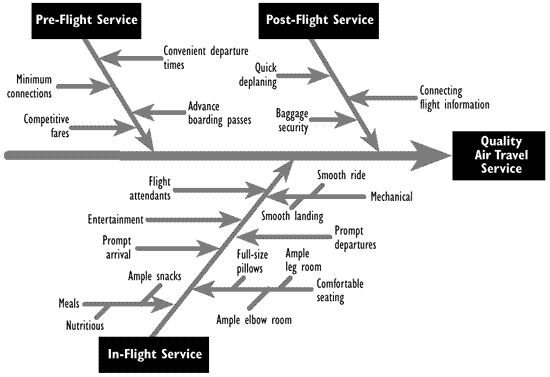
\includegraphics[width=10cm]{images/ishikawa_fishbone_diagram_example_itil.png}
    \caption{Example Ishikawa diagram for ITIL Service Support, \emph{Crown Copyright 2000}. \textbf{Will be replaced with one for this chapter.}}
    \label{fig:ishikawa_example_itil}
\end{figure}

Ishikawa diagrams, also known as fishbone diagrams, can help illustrate the relationships and relevance of various topics to the overall objective. Figure~\ref{fig:ishikawa_example_itil} is an example of an Ishikawa diagram for Service Support, with the aim of providing [good] quality air travel service~\cite{itil_ishikawa_example}. 

%%%%%%%%%%%%
% Learn more about Ishikawa diagrams
% https://www.moresteam.com/toolbox/fishbone-diagram.cfm 

\section{Topics to include in this chapter}
The following hierarchical list includes topics I plan to include in this chapter, after this section.


\begin{itemize}
    \item An overview on \emph{software quality}~\hyperlink{software.quality}{\emph{link}}
including various viewpoints of quality e.g. Gerry Weinberg)
    \begin{itemize} 
        \item ISO standards
        \item Software defects, faults and failures~\hyperlink{defects.faults.failures}{\emph{link}}
        \item QoE: Quality of Experience
        \item Classic references e.g. Phadke and perhaps Non-functional requirements in Software Engineering? 
        \item relevant / related academic research in my field
        \item Reliability. Introduced in ~\hyperlink{software.quality}{Software Quality}, and then expanded in a subsection~\hyperlink{software.reliability}{\emph{here}}
        \item Then focus on stability (as used by HP and then Google) encompassing reliability, freezes, etc.
        \item Discuss MTBF, usage paths and profiles and their effects on the measured values
    \end{itemize}
    \item Measurement and Analytics
    \begin{itemize}
        \item Views from outside software engineering e.g. how to measure anything book
        \item Software Analytics e.g. Buse and Zimmermann
        \item Sources and mechanisms for collecting data and information about mobile apps
        \begin{itemize}
            \item Human-centric sources e.g. ratings and reviews. Perhaps also discuss some of the flaws and limitations either here or in the 'caveats...' section later?
            \item Perhaps also consider in-app feedback c.f. the Mobile Twin Peaks paper?
            \item Alpha, Beta, Crowd, and other forms of testing with subsets of a population.
            \item Program-centric sources e.g. logging, crash reporting libraries, analytics libraries, platform-level observations.
        \end{itemize}
        \item Using Data
        \item Privacy and Control
    \end{itemize}
    \item Software Testing
    \begin{itemize}
        \item Schools of Software Testing? Old work that might help set the scene
        \item Classic references on software testing e.g. Boris Beizer
        \item using testing to measure quality and measuring software testing e.g. effectiveness.
    \end{itemize}
    \item App Stores and their effects on software development and engineering
    \begin{itemize}
        \item App Stores as ecosystems
        \item Release Planning (c.f DevOps and Release Engineering (including Shonan)
        \item Ratings and Reviews
        \item Google Play (and other Android app stores)
    \end{itemize}
    \item Developing mobile apps
    \begin{itemize}
        \item Single and multi-platform approaches
        \item A brief history of mobile app development
        \item Various species of bugs that affect mobile apps
    \end{itemize}
    \item Testing of Mobile Apps (this might be a distinct section in the Related Works as it's a rich topic). Do we care about testing of mobile apps that predates app store ecosystems?
    \begin{itemize}
        \item Automated testing frameworks and tools
        \item Testing practices (from both research and practical perspectives)
        \item Test Oracles
        \item Device Selection (as one aspect of testing for bug identification and investigation)
        \item Testing by crowds
        \item Measuring the efficacy of testing
    \end{itemize}
    \item Mobile Analytics~\hyperlink{mobile.analytics}{\emph{link}}
    \begin{itemize}
        \item types and sources of mobile analytics (also refer to appendix)
        \item Using Mobile Analytics to assess app behaviours
    \end{itemize}
    \item Caveats, constraints, flaws, limitations
    \begin{itemize}
        \item For instance on blind-spots, excessive trust and the ironies of automation. 
        \item Using crashes, ANRs, etc. as the test oracle - what will we miss if we only consider these aspects? how relevant is what we miss and what can we do to fill in some of the gaps?
    \end{itemize}
    \item Has anyone else published in my areas of research?
\end{itemize}

\hypertarget{software.quality}{}
\section{Software Quality}
Software quality is multi-faceted. Some facets are more user-centric, such as perceived quality by end-users, which may include aesthetics, responsiveness, brand perception, as much as more technical aspects such as whether an app freezes, crashes, or whether an app corrupts, leaks, or loses data, for instance. I cannot hope to %or it would be impractical and potentially counter-productive to
cover all the facets even after many years of working and researching in this domain. Instead I have selected the facets germane to my PhD research.

\textbf{TODO I need to explain why reliability is foremost.}
Several facets are able to be tracked remotely for mobile apps, an important factor in terms of the ability to facilitate practical approaches aimed at developers of these apps. They can be collected with various degrees of automation and to varying degrees, for instance the time something takes can be recorded at a micro level for a few lines of source code and at a macro level at the app or device level and across many devices and apps. 

There are well-established tools, techniques and practices for recording the time taken. Many of the tools are suited to use locally and directly by a developer, including Memory, App, and Network Profilers~\footnote{\url{https://developer.android.com/studio/profile\#android-studio-tools}}.For remote measurements the tools include Google's Android Vitals and Firebase Performance Monitoring\footnote{\url{https://firebase.google.com/docs/perf-mon}}.

User experience (UX) can be assessed using a wide variety of tools and techniques, such as heatmapping (which uses screen and/or interaction recording), A/B testing frameworks, funnel and journey analytics, and so on. By their very nature they're user-focused and - in practice - seldom incorporated into mobile apps or development practices for mobile apps. Similarly, based on my investigations, they are seldom researched although I have co-written work on this topic including examples of using heatmapping to improve usability of mobile apps~\cite{harty_aymer_playbook_2016}.

\yy{Logically I don't see the connection between quality facets => quality (general) => reliability (facet) again, perhaps you want to add some transitions so readers can follow the thoughts.}

Crash data is impersonal and oft requested and collected by operating systems and applications. For instance, when an Apple operating system is updated users are asked a couple of questions including whether they are willing to share crash data with Apple and with developers [of apps].

Weinberg stated \emph{"Quality is value to some person"}~\cite{weinberg1992quality}. To paraphrase him, \emph{Quality is in the eye of the beholder}.

\akb{You will need to choose an existing taxonomy of software quality and explain which aspects are relevant to your research before discussing literature from each of these aspects. The Kitchener et al paper below is a good starting point for this.}

\subsection{Papers to consider}

\begin{itemize}
    \item "Software Quality: The elusive target"~\cite{kitchenham1996_software_quality_elusive_target}. - \emph{'So how do we assess ``adequate" quality in a software product? The context is important.'}, \emph{"A good definition [of software quality] must let us measure quality in a meaningful way. Measurements let us know if our techniques really improve the software, as well as how process quality affects product quality."}
    \item "Cornering the Chimera"~\cite{dromey1996_cornering_the_chimera}.
    \item "QoE Doctor: Diagnosing Mobile App QoE with Automated UI Control and Cross-layer Analysis"~\cite{chen2014qoe}.
    \item "An Approach to Detect Android Antipatterns"~\cite{hecht2015approach}. Using static analysis to find poor designs that lead to poor quality apps. Their approach could be complementary to mine and to software testing.
    \item ...
\end{itemize}

\subsection{Seven Quality Control Tools}
Ishigawa's work extended beyond the eponymous Ishigawa, or fishbone, diagram (as illustrated in Figure~\ref{fig:ishikawa_example_itil}); he also devised seven basic tools for quality, in turn inspired by W. Ewdards Deming's lectures in Japan in the 1950's~\cite{7_basic_quality_tools_with_R}.

Of these seven tools, two are of particular interest in my research, his diagram to help set this work in context, and Pareto charts (also known as the Pareto distribution diagram), illustrated in one of the appendices~\hyperlink{pareto.diagrams.in.r}{\emph{here}}.

Reliability is one facet of software quality, and a measure of how reliable (error-free) software is in use. \yy{Why do you focus on reliability as the only facet of quality after dismissing the other facets? Do you need to worry about correctness as another quality facet related to testing?} 

\hypertarget{defects.faults.failures}{}
\subsection{Software Defects, Faults and Failures}
\emph{Add a preamble to why this subject is relevant to my research - set this topic in context. Keep the examiner on the read thread of my research.}
\yy{The heading doesn't match yet with the content: what about Faults and Failures? You may consider this standard for one definition:
\url{https://ece.uwaterloo.ca/~agurfink/ece653/assets/pdf/W01P2-FaultErrorFailure.pdf}}
According to Mäntylä and Itkonen more defects were found implicitly (62\%) than explicitly (38\%) ~\cite{mantyla2014_how_are_software_defects_found}, based on a survey of four software development companies in three different companies. The authors state \emph{"Implicit defect detection has a large contribution to defect detection in practice, and can be viewed as
an extremely low-cost way of detecting defects."}. Similarly my research may be considered as a useful source of finding defects implicitly, where the defects are mined and reported by mobile analytics tools and development teams can decide on the defects they deem sufficiently relevant \emph{and} practical to fix. I will discuss separately some of the implications of applying this approach to complement other approaches.

\emph{Add the take aways of why I've included this topic. Be clear about why using analytics is different from what's been done before. Explain the gaps in prior work}

~\hypertarget{software.reliability}{}
\subsection{Software Reliability}
Over twenty years ago, in a paper published at ICSE in 1997, the authors (Frankl, Hamlet, and Littlewood) discussed approaches to select testing methods to deliver reliability. They identified two main goals in testing software: 
\begin{enumerate}
    \item to \emph{achieve} reliability~\cite{frankl1997choosing_testing_for_reliability} (using testing to probe software for bugs so they could be removed to improve the reliability), and 
    \item to \emph{evaluate} reliability, an approach they call \emph{operational testing}, where tests reproduce the expected usage of software and testers wait for failures to occur.
\end{enumerate}

Both approaches provide a mixed bag of desirable and undesirable effects; in the paper the authors compare the testing effectiveness based on the reliability of the program after it was tested. In their conclusion they state: \emph{"research cannot offer decision makers a best testing method for all situations."}. Instead they believe research can offer better criteria for informing the choice of a method to suit a decision maker's specific situation. They also hope to guard against, and help people avoid, illogical decisions.

Their work intersects with the work of Dorothy Graham's proposed measure of Defect Detection Percentage (\emph{DDP}, for short)~\cite{graham_measuring_2009} aimed at evaluating the effectiveness of whatever testing was performed by comparing the issues found during testing with those found subsequently, often when the software is in use by others.

Frankl, Hamlet, and Littlewood discussed operational testing based on expectations of the inputs; in turn a paper by Bishop in 1993~\cite{bishop1993variation} discussed the variation in software survival time depending on differences in the operational input profiles. Failure probabilities are not constant, the paper states the probability of failures decreases as the time from the last failure increases. There are several relevant observations in the paper, including: \emph{"During a failure, restarting the software will have little effect if the input conditions are similar..."} for instance a mobile app may crash repeatedly if a user (for instance) happens to repeat an action that exercises the code that fails. I observed this behaviour in Kiwix, one of the Android apps under evaluation, where a single crash occurred 55 times for a single user.\yy{It is good to confirm the points in your observation.}

Another result from the paper is: \emph{"Given that the software is operating successfully, the chance of continued operation is greatly improved if there are only small changes in input conditions..."}. For mobile apps, one of the ongoing, major, sporadic changes are to the version of the operating system. As \textbf{TODO add link to API fault proneness paper} found, the most frequent cause of failure for Android apps is when the operating system is updated. Apps that were reliable on previous releases of the operating system may now start failing, and some failures become frequent and widespread as the new operating system release is adopted. \textbf{TODO add evidence on the rollout and growth of Android releases in use as per old Google Android charts.}\yy{This is very true in the TM352 I experienced. An argument may lead to the gap analysis is: how can one control or limit the effect of such external change factors or live with it? Is mobile analytics towards living with it while presenting an opportunity to spot such incompatibility issues earlier? }

These existing works help to establish the importance of reliability, some of the ways testing can be evaluated in terms of the subsequent reliability of the software in use, and some of the challenges in finding bugs that affect reliability. 

\textbf{TODO} sum up this section and connect it with Google's concept of Stability metrics to measure software quality for Android apps.

\section{Measurement and Analytics}

\begin{figure}
    \centering
    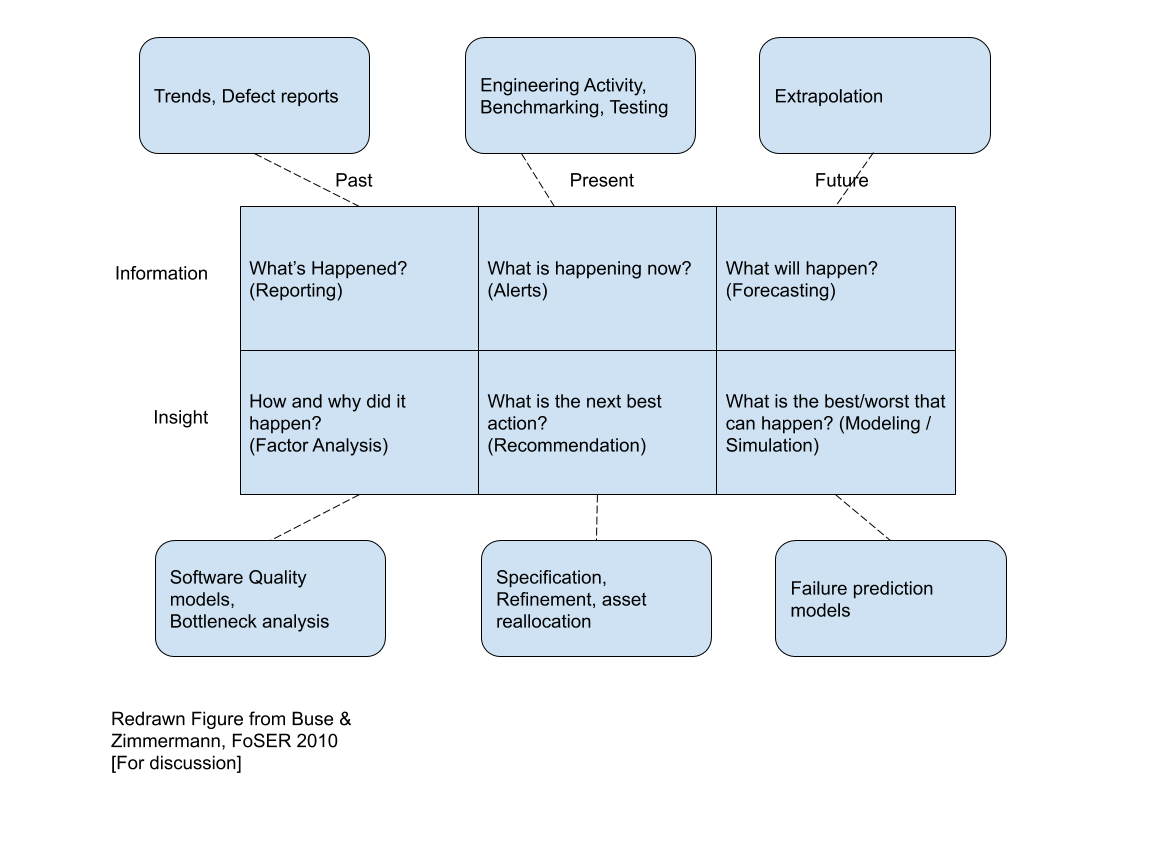
\includegraphics[width=14cm]{images/Buse_and_Zimmermann_2010_figure.png}
    \caption{Software Analytics, Buse and Zimmerman (2010)}
    \label{fig:software_analytics_buse_and_zimmerman_2010}
\end{figure}

\subsection{Papers to consider}
\begin{itemize}
    \item Buse and Zimmermann... 
    \item     
    \item "A Methodology and Framework to Simplify Usability Analysis of Mobile Applications" Adding logging to a mobile apps can help developers analyse usability, reducing the effort needed
\end{itemize}

\subsection{Topics to mention}
\begin{itemize}
    \item Use of analytics is ubiquitous by software, including operating systems (e.g. OSX), mobile platforms (including Android and iOS), web servers, and mobile apps. 
    \item Understand what's being measured, and what's being claimed. e.g. Zoom corrected their claims about their user-base for their progress report on \nth{22} April 2020 \emph{even with more than 300 million daily meeting participants.}, they acknowledged they'd previously stated the claimed meeting participants were users and people \emph{"Edit 4/29/20: This blog originally referred to meeting participants as “users” and “people.” This was an oversight on our part."}~\footnote{~\url{https://blog.zoom.us/wordpress/2020/04/22/90-day-security-plan-progress-report-april-22/} and see the commentary in the ITPro article:~\url{https://www.itpro.co.uk/marketing-comms/communications/355498/zoom-quietly-corrects-misleading-claims-of-over-300-million}}
    \item Ways data can be used
    \item Privacy, and who is responsible for the data being collected, shared, and protected?
\end{itemize}


\subsection{Development Logging}
Consider a 2D matrix of use of logging (amount, choice of library and API, formatting and customisation), and the range of the logging (local<->logging at a distance). Papers such as \emph{A Methodology and Framework to Simplify Usability Analysis of Mobile Applications}~\url{https://doi.org/10.1109/ASE.2009.12}. Remember to cover this topic in the work we did on logging (And the recent Shonan work). Mention the Shonan workshop in this section too.

\subsubsection{Use of logging}

\subsubsection{Research in logging}

\subsubsection{Designing logging}

\subsection{Ubiquitous Analytics}
After OSX operating system updates, and when new users first login, they are asked to "help app developers improve their products and services automatically." Tickbox, default un-selected: "Share crash and usage data with app developers", "Help app developers improve their apps by allowing Apple to share crash and usage data with them." Further details, including from a user's perspective what's collected, how long the data is kept, and how to disable diagnostics from being sent are all described in \url{https://support.apple.com/en-gb/guide/mac-help/mh27990/mac}

\subsection{Ways data can be used}
In Industry there are discussions on various ways data can be used to get the most out of the data. Figure~\ref{fig:i_am_using_data_to} presents a decision tree discussed in an article on when to apply each perspective~\cite{amplitude_are_you_data_driven}. For my research, and for development teams who use analytics, we may choose to use these various perspectives to use analytics data more productively. This work leads to the question of identifying and often designing the data that will need to be collected in order to use it.

\begin{figure}[ht]
    \centering
    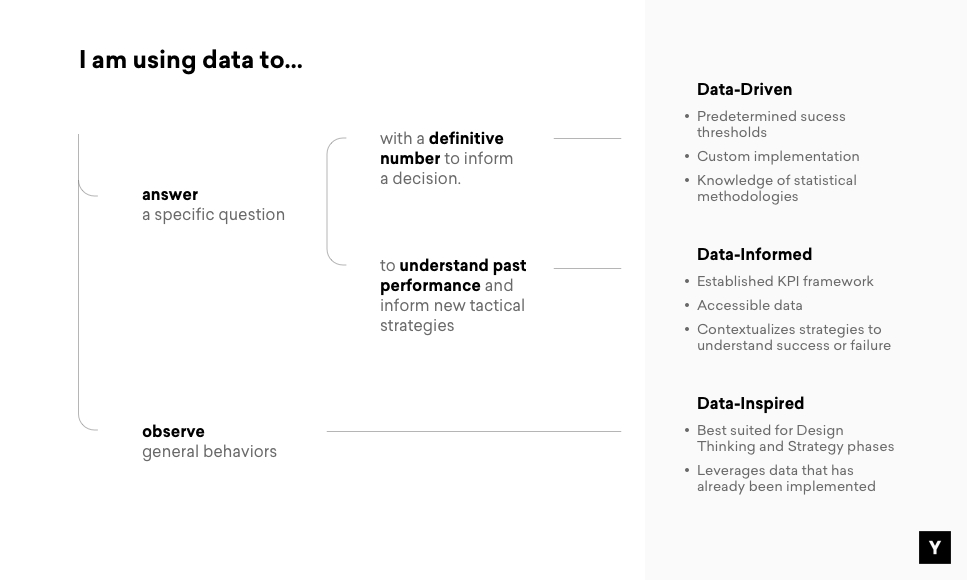
\includegraphics[width=15cm]{images/data-informed-graphic-ymedia-labs.png}
    \caption{I am using data to... (from Y Media Labs)~\cite{amplitude_are_you_data_driven}}
    \label{fig:i_am_using_data_to}
\end{figure}
%First discovered via \url{https://twitter.com/iteratively/status/1243641701408935936?s=20}

Identifying and designing data....


\subsection{Privacy and Control}

UW blog post~\cite{mcquate_I_saw_you_were_online} and the underlying CHI 2020 paper~\cite{cobb2020_ux_s_with_online_status_indicators} regarding how online status indicators shape their behaviour and on whether people know and can correctly control whether their data is being shared.

c.f. using infra-red cameras to detect people in ways they're unfamiliar with and do not expect. 

\section{Software Testing}

\subsection{Papers to consider}
\begin{itemize}
    \item TBC
    \item Behaviourally Adequate Software Testing \url{https://leicester.figshare.com/articles/Behaviourally_Adequate_Software_Testing/10106189} - Behavioural Coverage, search-based white-box generation strategies. Measures of testing adequacy. \emph{One intuitive notion of adequacy, which has been discussed in theoretical terms over the past three decades, is the idea of behavioural coverage; if it is possible to infer an accurate model of a system from its test executions, then the test set must be adequate.} IIRC the programs they assess are tiny, and how can we determine 'accurate model', perhaps it'll be accurate for what it tests, but incomplete? "The truth, \emph{the whole truth}, and nothing but the truth" springs to mind. % See also Uncertainty-Driven Black-Box Test Data Generation (seems less relevant to my research) and Assessing Test Adequacy for Black-Box Systems Without Specifications (perhaps more relevant).
    \item "Probably approximately correct learning" however it seems to be unrealistic and impractical for shipping mobile app development teams.
\end{itemize}


\subsection{Concepts to consider}
\begin{itemize}
    \item Adequacy
    \item Confidence levels (in the testing we've done)
    \item Sufficiency (c.f. how Google graded OKRs where 0.7 was the expected, sufficient, amount of progress).
    \item What testing actually gets done for real software, rather than what testing standards, academia, etc. tells us we \emph{should} do.
    \item Probably Approximately Correct.
\end{itemize}

\section{App Stores and their Effects on Software Development and Engineering}

\subsection{Papers to consider}
\begin{itemize}
    \item \textbf{"A survey of app store analysis for software engineering"}~\cite{martin2016survey}.
    
    \item \textbf{"Why people hate your app: Making sense of user feedback in a mobile app store"}~\cite{fu2013people}. A key paper, many citations (some also highly relevant).
    
    \item "Analyzing and Automatically Labelling The Types of User Issues that are Raised in Mobile App Reviews"~\cite{mcilroy2016analyzing} - discusses crashes, crash libraries, analytics, relatively early paper on the topic.
    
    \item \emph{``Revisiting the Mobile Software Ecosystems Literature"}~\cite{steglich2019revisiting} Helps to define what an ecosystem is.
    
    \item "Beyond Google Play: A large-scale comparative study of Chinese Android app markets"~\cite{wang2018beyond}.
    
    \item "Measurement, modeling, and analysis of the mobile app ecosystem"~\cite{petsas2017measurement}.
    
    \item "A Measurement-based Study on Application Popularity in Android and iOS App Stores"~\cite{liu2015measurement}.
    
    \item "Understanding the Evolution of Mobile App Ecosystems: A Longitudinal Measurement Study of Google Play"~\cite{wang2019understanding} (2019): Lots of interesting questions and observations about Google Play; but they don't seem to consider flaws, or the effects of flaws, in the app store's data collection, algorithms, etc.
    
    \item \emph{``Release Practices for Mobile Apps--What do Users and Developers Think?"}~\cite{nayebi2016release}.
    
    \item \emph{``Feature lifecycles as they spread, migrate, remain, and die in App Stores"}~\cite{sarro2015_feature_lifecycles_in_appstores} discusses \emph{adaptive development} as a concept for developers of apps in app stores. Notes: Their research is based on `non-free features from two app stores (Samsung and Blackberry)' (both relatively dwarfed by Google Play) and their work predates the availability of platform level analytics, etc. Relevance to my work: developers can obtain requirements (in terms of work they're potentially `required' to do) from many sources, including direct feedback from end users of the apps, signals in terms of willingness to install and keep using their app, and from analytics. Developers want and increase the value of their work by prioritising potential work appropriately. Signals and data from mobile analytics may provide useful, additional sources of information that's sufficiently relevant for developers to accept these `requirements' and address them.
    
    \item \emph{``Which version should be released to app store?"}~\cite{nayebi2017version}.
    
    \item \emph{``Modern release engineering in a nutshell - why researchers should care"}~\cite{adams2016modern}.
    
    \item The \emph{``Data analytics for decision support in software release management"}~\cite{didar2018data_analytics_phd_thesis}, a PhD thesis, introduces a proposed Plan-Monitor-Improve Framework for release management.
    
    \item \emph{"An Explorative Study of the Mobile App Ecosystem from App Developers' Perspective"}~\cite{wang2017_exploratory_study_of_the_mobile_app_ecosystem}: 1,000,000+ apps on Google Play, 320,000 developers, over half of the developers only released a single app. The paper mainly focuses on the \emph{"the group of aggressive developers who have released more than 50 apps, trying to understand how and why they create so many apps"}. Provides some context on who writes the mobile apps in Google Play, provides an estimate of the population of developers (in 2017).
    
    \item \emph{``Requirements Intelligence: On the Analysis of User Feedback"}~\cite{stanik2020requirements_intelligence_on_the_analysis_of_user_feedback}. continuous sources for requirements-related information; comparison between explicit and implicit user feedback (like app usage data).
    
\end{itemize}


App Stores behave as intermediaries between developers and the users of their software. They make various aspects more transparent including pricing, information about the apps, releases, and ratings \& reviews. There are hundreds of thousands of developers of Android apps according to various sources (320,000 in 2017~\cite{wang2017_exploratory_study_of_the_mobile_app_ecosystem}, ...).


In an App Store first the developer then the app store are involved in making a release available to some or all of the user population. There are various competing factors that affect when would be a good time to make a release. Too few and an app may be considered stale or neglected, too many and users may balk at the seemingly endless updates and communications costs. Groups of researchers have investigated various aspects of release engineering, including~\cite{adams2016modern} that argues the relevance of modern release engineering and the relevance for researchers, and~\cite{nayebi2017version} which concentrates on which version of opensource apps should have been released to the app store. Developers, and their stakeholders, want to make more informed decisions about which releases to make; however there does not appear to have been much research into the testing and quality indicators available to app developers before they make their release public.


\section{Developing Mobile Apps}

\subsection{Papers to consider}
\begin{itemize}
    \item TBC
    \item \textbf{Species of Bugs}
    \begin{itemize}
        \item "Finding resume and restart errors in Android applications"~\cite{shan2016finding}. Which leads to "Large-scale analysis of framework-specific exceptions in Android apps" (2018) where the exceptions should be detectable by Android Vitals, I hope.
    \end{itemize}
\end{itemize}

\subsection{Bugs}
Species of bugs: data loss bugs: When apps lose data they also lose the trust of users. One cause of data loss in Android apps has been investigated recently (2019) in ~\cite{riganelli2019benchmark_android_data_loss_bugs} where the authors found 19.2\% of the Android apps they evaluated lost data. The data losses were of one particular type - where the app failed to save and/or restore data when the app was stopped and restarted. There are other causes of data loss for mobile apps including database, network and storage errors, for example. They claim some of these bugs may surface as crashes in the app at a later stage, after the data was lost and the app resumed, however their examples did not seem to result \yy{in} crashes. \yy{Data loss is definitely a sign of lack of integrity. Sometimes it is required to lose some user data for privacy protection. Maybe you can refine the definitely more precisely to refer to "retaining the data that users care".} \yy{I think one of the gaps is that the data loss bug that does not lead to crashes are actually bugs too. This is kind of important to justify your work will be different from other app testing literature that focus on detecting crash related bugs.}

To the authors' credit they provide extensive material including automated tests for the vast majority of the bugs~\footnote{\url{https://gitlab.com/learnERC/DataLossRepository}}. They were able to create automated tests that reproduced 110 of the 116 errors and were able to automatically detect 98 out of the 110 errors they were able to reproduce.

One of the considerations this work helps to illustrate is the many challenges of measuring software quality comprehensively, or even adequately.

\textbf{TODO} Wrap up this sub-section with where most of the research has been in terms of bugs in mobile apps.

\hypertarget{mobile.testing}{}
\section{Testing Mobile Apps}

\subsection{Papers to consider}
\begin{itemize}
    \item "Mobile Testing-as-a-Service (MTaaS)--Infrastructures, Issues, Solutions and Needs"~\cite{gao2014mobile}. This paper, published in 2014, in my view isn't particularly novel. Rather it summed up stuff that was happening in industry at the time and combined it with a bunch of ideas of what \emph{might} be worth doing in the authors' view. The aim of the authors is to set the direction for scaling testing of mobile apps. Six years on is a good time to assess their suggestions.
    \item "The Testing Method Based on Image Analysis for Automated Detection of UI Defects Intended for Mobile Applications". \textbf{Springer paper I paid for.}
\end{itemize}

\hypertarget{mobile.analytics}{}
\section{Mobile Analytics}

\subsection{Papers to consider}
\begin{itemize}
    \item TBC
\end{itemize}

Direct vs indirect analytics - 
Challenges of research into usage-derived analytics - perhaps why there are gaps in knowledge, compounded for indirect analytics. A tale of two apps, any others?
